\documentclass[11pt]{scrartcl}

\usepackage{geometry}                % See geometry.pdf to learn the layout options. There are lots.
\geometry{letterpaper}                   % ... or a4paper or a5paper or ... 

\usepackage[parfill]{parskip}    % Activate to begin paragraphs with an empty line rather than an indent

\usepackage{amssymb}
\usepackage{fixltx2e}
\usepackage{hyperref}
\usepackage{graphicx}
\DeclareGraphicsRule{.tif}{png}{.png}{`convert #1 `dirname #1`/`basename #1 .tif`.png}
\graphicspath{{./figures/}}

\begin{document}

\title{Diffusive Programming}
\subtitle{Simplifying Task-Oriented Distributed Computing}
\author{Robert Philipp}
\date{\today}
\maketitle

%
% abstract
%
\begin{abstract}
The goal of \emph{diffusive programming} is to make task-oriented distributed computing easier by separating the execution logic from the distribution logic. \emph{Diffusive programming}, defined by a set of six principles, is an approach for performing method-level, task-oriented distributed computing. In \emph{diffusive programming}, any method can be \emph{marked} for distribution, regardless of its signature. And \emph{marking} a method is necessary and sufficient for its execution to be distributed. Distribution of tasks occurs through a network of nodes that can accept tasks and execute them, or forward them on. Nodes executing a task, load the required resources as needed, and cache them. The topology of the network of nodes can be anything that can be represented as a directed graph. Topologies can be tailored to solve specific problems. \emph{Diffusive} is a Java reference implementation of the six principles that define \emph{diffusive programming}.
\end{abstract}

%
% introduction
%
\section{Introduction}
Task-oriented distributed computing allows independent computational tasks to be distributed to multiple computing nodes, presumably to execute in parallel. This approach can reduce the overall compute time of a set of independent tasks. For example, in quantitative finance, one may desire to calculate risk metrics for each financial instrument contained in a large portfolio. When the calculation of the desired risk metrics for each instrument is independent of the calculation for all other instruments, the risk metrics of each instrument can be calculated independently. In this case, we can speed up the risk metrics calculation for the portfolio by spreading these independent tasks over many compute nodes at once, and then collecting the results.

Typically this type of distribution is performed by a distribution middleware. In many cases, the application makes calls to the middleware's application programming interface (API). The computational task may be represented by an object whose class implements an interface that represents a \emph{compute task} as defined by the middleware. Including middleware API calls in the application code couples the application to the middleware. And more concerning, the application is now polluted with code used to distribute execution to remote compute nodes. Clearly, with careful design, much of that distribution logic can be hidden behind wrappers that allow the application logic to interact with an abstract compute engine, instead. And, the compute engine could be implemented to execute locally or remotely. But even this approach doesn't overcome the constraints imposed by the requirement that computational tasks implement a specific interface\footnote{Typically, a \textsf{Task} interface would contain an equivalent to an \textsf{execute(...)} method. That means that any task that is to be distributed must adhere to the signature of that \textsf{execute(...)} method. And conversely, the signature of that \textsf{execute(...)} method must be general enough to support any task.}.

Distribution middleware may also require deployment of certain resources (dynamic libraries, class files, etc) to the compute nodes \emph{before} they can execute remote requests. This requires careful synchronization of versioned resources. And this renders the compute nodes generic, only insofar as the required resources have been deployed to that node.

\emph{Diffusive programming} is based on a set of six principles intended to facilitate the development of task-oriented distributed applications. it is an approach for performing task-oriented distributed computing that allows the execution of individual methods to be distributed. Any method can be distributed, regardless of its signature. And aside from specifying that a method is to be distributed, no further code changes are required. Furthermore, \emph{Diffusive programming} allows the application code to define the execution logic (i.e. the order and concurrency of the execution threads) without having to explicitly implement how tasks are distributed---the implementation of the \emph{diffusive programming} principles manages the distribution of \emph{marked} methods.

Section \ref{sec:principles_of_diffusive_programming}, \textit{\nameref{sec:principles_of_diffusive_programming}}, provides a concise version of the principles and defines additional terms used throughout the rest of the paper. Its subsections, \ref{sec:marking} through \ref{sec:open_topoloogy}, describe each principle in more detail. With the principles defined and explained, section \ref{sec:diffusion_patterns}, \textit{\nameref{sec:diffusion_patterns}}, puts forth a few network topologies, or patterns, that are possible through diffusive programming. And section \ref{sec:reference_implementation}, \textit{\nameref{sec:reference_implementation}}, describes \emph{Diffusive}, the Java reference implementation of the \emph{diffusive programming principles}. Finally, section \ref{sec:future_work}, presents future work to be done on diffusive.

%
% Principles of diffusive programming
%
\section{Principles of Diffusive Programming\label{sec:principles_of_diffusive_programming}}
\emph{Diffusive programming} is based on six principles that define a framework for performing task-oriented distributed computing. The six principles are ordered. They build on each other, progressing from the action of distributing the code to the deployment and configuration of the computation nodes.

\subsection{The Principles}
\begin{description}

	% marking, diffusive
	\item[Marking] 
	A method can be marked for remote execution. The act of \emph{marking}, alone, is sufficient and necessary for a method to be executed on a remote location and have the results returned.
	
	\emph{Definition}: A \textbf{diffusive} method is a method that has been \emph{marked}.

	% location opaquenes
	\item[Location Hiding]
	Code calling a \emph{diffusive} method does not, and can not, know on which resource that method was executed. This helps keep code \emph{cohesive} by removing distribution logic from the application. 
	
	\emph{Definition}: A \textbf{diffuser} is what executes a \emph{diffusive} method.
	
	\emph{Definition}: A \textbf{diffused} method is a \emph{diffusive} method that was executed by a \emph{diffuser}. 
	
	% failure hiding
	\item[Best-Efforts Failure Resolution]
	A \emph{diffuser} will attempt to recover from a \emph{diffusive failure}. If the \emph{diffuser} is unable to recover, it will transfer error handling to a specified handler or report the error as a local error.
	
	\emph{Definition}: A \emph{diffusive failure} is a the failure of a remote \emph{diffuser} to execute a \emph{diffusive} method, or the loss of connectivity to a remote \emph{diffuser}.
	
	% generic computation engine
	\item[Generic Computation]
	Any \emph{diffusive} method can be executed by any \emph{diffuser}. A \emph{diffuser} need not be configured with resources prior to the request to execute a method.
	
	% indistinguishablity
	\item[Indistinguishability]
	A \emph{diffuser} is responsible for executing any \emph{diffusive} method, and it is also responsible for \emph{diffusing} methods to other \emph{diffusers}. This implies that a \emph{diffuser} must be able to act both as a client and and as a server.
	
	% open topology
	\item[Open Topology]
	\emph{Diffusers} can be connected in any topology that can represented as a directed graph. Each node in the directed graph represents a \emph{diffuser}. Each directed edge represents a connection from one \emph{diffuser} to another. The direction of the edge represents the direction of the \emph{diffusion}. And, each \emph{diffuser} may contains connections to a set of other \emph{diffusers}. 
	
	\emph{Definition}: A \emph{diffuser network} is a set of connected \emph{diffusers}.
	
	\emph{Definition}: Suppose we have two \emph{diffusers}, \textbf{A} and \textbf{B}. We say that \textbf{B} is an \emph{end-point} of \textbf{A}, if \textbf{A} \emph{diffuses} methods to \textbf{B}.

\end{description}

The following subsections describe each principle in more detail, and where applicable, how that principle differs from more typical or traditional methods of distributed computing.

% marking
\subsection{Marking\label{sec:marking}}
\emph{Diffusive programming} allows the execution of individual methods to be distributed. \emph{Marking} a method is the act of specifying that a specific method is to be distributed. How a method is \emph{marked} is up to the implementation of this principle. However, this principle does state that the act of \emph{marking} a method is necessary and sufficient for the method to be distributed. This means that \emph{any} method can be marked, and, therefore, executed, regardless of its name, parameters, or return type. This is a departure from many typical task-orient approaches that require the implementation of task interfaces, where the method to be executed has a defined signature (and return type).

The way a method is marked, to become a \emph{diffusive} method, depends on the implementation of this principle. For example, the reference implementation written in Java currently uses annotations to mark methods. However, it could just as easily allow the fully qualified method names to be specified in a configuration file instead.

The act of marking a method decouples the distribution logic from the application logic. And this leads us to the next principle: location hiding.

% location hiding
\subsection{Location Hiding\label{location_hiding}}
\emph{Marking} a method tells the diffusive framework that that method is to be executed in a distributed manner. But it is the principle of \emph{location hiding} that places the requirement that any code calling a diffusive method does not know, or need to know, where that method is executed. Removing the responsibility of knowing or having to deal with the consequences of where the method is executed relieves the calling code of any responsibility regarding distribution. And this allows the application code to remain cohesive. It also means that the same code can be called in a distributed manner, or to run completely locally with any change to the application logic.

In typical distributed systems, the distribution logic must be called directly from the application code. This may occur by calling low level application programming interfaces (API) such as in MPI, or writing task classes that implement interfaces defined by the distribution framework, and then modifying application code to deliver these tasks to the middleware.

Location hiding allows code to be endowed with its execution logic, and that execution logic is then automatically mirrored, but in a distributed manner, simply by marking the method(s). When this is coupled with the next principle, \emph{generic computation}, we have a powerful and simple mechanism to distribute computation.

% best efforts failure resolution
\subsection{Best-Efforts Failure Resolution\label{sec:best_efforts_failure_resolution}}
A task that is called and executed completely within a local address space\footnote{For example, code running entirely in one process.} may fail to return a result. The failure may occur because an input or logic error, and in this case, it may be possible to trap and handle the error condition. In other cases, the failure may occur because of an unanticipated bug\footnote{As opposed to the anticipated bug.} or because the server crashed. Under these conditions it may not be possible to trap and handle the error condition, and the entire application may crash or become unresponsive. In both scenarios, however, the fact that there was a failure is known\footnote{Either to the code trapping the error, or the user because the application crashed.}.

The situation may be quite different when a task is called from one address space and executed in another. For example, suppose the application-attached diffuser diffuses a method to a remote diffuser. Now suppose further that the task fails to execute because of an input or logic error. If the remote diffuser traps the error, it could return an error condition which is return, and again trapped by the application-attached diffuser, and handled as in the non-distributed case. However, suppose instead that the input or logic error isn't trapped, or if there is a bug that causes the task to crash, or if the server crashes, or if the network connection goes down. In this case, the application-attached diffuser waits for the result, but doesn't receive one. Yet, the application-attached diffuser doesn't know if the task is still executing, or if there was a failure.

The \emph{best efforts failure resolution} principle requires that the application doesn't see a difference between a purely local and a distributed failure. The diffuser making the request is expected to perform its best to recover from a \emph{diffusive failure}, and if it can't, then it reports the error. For example, diffusers could provide a status service that responds if the diffuser is running and accessible. If the requesting diffuser finds that the status of the remote server is down, then it diffuses the method to a different diffuser. It may attempt to send the task to a different diffuser a configured-number of times before giving up and reporting an error.

% generic computation
\subsection{Generic Computation\label{sec:generic_computation}}
The principle of \emph{generic computation} provides that any method can be executed on a \emph{diffuser} without out the need to deploy the resource needed to execute that diffused method. Simply put, the shared object libraries or classes don't need to be deployed to the remote server prior to making the request. Each \emph{diffuser} must contain a mechanism for providing resources to remote locations and for loading resources from a remote location.

In typical distributed computing, required resources must be deployed to the remote servers prior to requesting remote execution of a specific task. Diffusive programming removes this restriction by requiring that the mechanism which distributes the method execution also provides a capability to deliver the required resources to execute the method. 

Note that, however, this does not prevent users from deploying resources to a common location from which they can be obtained at run-time. Under certain deployment scenarios, it may be desirable to have such a common location to provide a centralized control over the versions. But even in this case, the resources need only be deployed to the one common area.

% indistinguishability
\subsection{Indistinguishability\label{sec:indistinguishability}}
The principle of \emph{indistinguishability} means that a \emph{diffuser} must be able to receive requests to execute, and at the same time be able to \emph{diffuse} (forward) those requests to another \emph{diffuser}. In other words, there isn't such a thing as a client diffuser and a server diffuser: they are one and the same.

The \emph{generic computation} principle alluded to this principle of \emph{indistinguishability}. The generic computation principle states that a diffuser must be able to load resources from a remote diffusers, \textbf{and} at the same time must be able to provide resources to a remote diffuser.

% open topology
\subsection{Open Topology\label{sec:open_topoloogy}}
The \emph{open topology} principle, coupled with the \emph{indistinguishability} principle, requires that it is possible to create networks of \emph{diffusers}, called \emph{diffuser networks}, in any topology that can be represented as a directed graph. Each node in the directed graph represents a \emph{diffuser}, and each (directed) edge connects that \emph{diffuser} to an \emph{end-point}, which is another \emph{diffuser}. Any network that can be represented by a directed graph can be constructed. 

This principle allows the construction of networks tailored to solve specific or general problems, networks that can naturally learn/discover an optimal configuration for performing certain types of tasks, or networks that contain sufficient redundancy to provide execution within required timelines. Section \ref{sec:diffusion_patterns}, \emph{\nameref{sec:diffusion_patterns}}, describes a few possible network topologies (patterns) that are designed to solve specific problems.

%
% Diffusion patterns
%
\section{Diffusion Patterns}\label{sec:diffusion_patterns}
\emph{Diffusion patterns} are made possible by the last three diffusive programming principles: generic computing; indistinguishability, and open topology. Together, these three principles make the statement that \emph{diffusers} form building blocks that can be connected as directed graphs. The principle of \emph{open topology} requires that a diffuser be connected to zero or more end-points to which it can diffuse execution of a method. The principle of \emph{indistinguishability} states that each end-point, itself, must be a diffuser. This means that that diffuser itself is connected to zero or more other end-points. And, therefore, it can receive tasks as well as diffuse them. Finally, the principle of \emph{generic computing} requires that a diffuser be able to receive (and send) resources needed to execute a task, allowing tasks to be diffused to other nodes dynamically and executed.

Because any diffuser network that can be represented as a directed graph is possible to construct, there are an infinite number of patters in which these networks can be constructed. And furthermore, their dynamic nature also allows the networks to evolve over time. In the next subsections I describe three illustrative patterns that solve specific problems.

Finally, it is important to emphasize that it is the \emph{marking} principle and the \emph{location hiding} principle that require the diffusive framework to provide a mechism for intercepting \emph{marked} method calls and handing them to the (local) diffuser assigned to the application. It is that (local) diffuser that then takes care of diffusing the execution of the \emph{marked} method to other remote diffusers for execution. Therefore, all the topologies have this characteristic in common.

% layer network topology
\subsection{Layered}
The layered topology is the simplest, and most similar to many distributed middleware solutions. In this topology, the diffuser collocated with the application, which we will call the \emph{application-attached diffuser}, is connected to a set of end-points, which we call the \emph{remote diffusers}. The application-attached diffuser, depending on the specifics of its configuration, is responsible for distributing the tasks to the the remote diffusers. The remote diffusers execute the task and return the results to the application-attached diffuser, which returns the results to the application\footnote{In the discussion about the reference implementation, \emph{Diffusive}, I'll provide details on how these steps can be implemented.}. 

\subsubsection{Single Layered}
Figure \ref{fig:topology_single_layer} shows the simplest topology---a single layered diffuser network. In this figure, the circles label with \textbf{D} are \emph{diffusers}, the square at the bottom label with \textbf{A} is the application containing the methods to be diffused. In this topology, the application-attached diffuser is responsible for distributing the tasks to the remote diffusers. The remote diffusers execute their assigned task and return the result to the application-attached diffuser, which then returns it to the application.

\begin{figure}[htbp]
\begin{center}
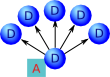
\includegraphics[scale=1.0]{topology_single_layer}
\caption{Single Layer Diffuser Network Topology\label{fig:topology_single_layer}}
\end{center}
\end{figure}

Although not covered in the diffusive principles, because it is an implementation detail, it is worth noting at this point that any implementation must address the strategy used to distribute the tasks amongst the diffusers---local and remote. The reference implementation \emph{Diffusive} provides a \textsf{Strategy} interface that can be implemented to provide a specific strategy based on CPU load, number of executing threads, weighting, or some other scheme. Clearly, the implementation of such a strategy will effect the performance characteristics of the diffusive network.

\subsubsection{Multi-Layered}
A natural extension of the single-layered diffuser pattern is a multi-layered diffuser pattern. One such pattern is  shown in figure \ref{fig:topology_multi_layer}. Implementations of the diffusive principles that allow nested method \emph{marking} allow tasks to be diffused that, themselves, contain subtasks that are to be diffused, which is essentially map-reduce. This type of topology can dramatically improve the performance of calculations that can be represented as tasks of subtasks. An illustrative example is a calculation that is composed of a set of independent calculations, where each of these independent calculations are themselves composed of a set of independent calculations. 

\begin{figure}[htbp]
\begin{center}
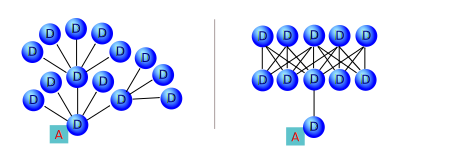
\includegraphics[scale=1.0]{topology_multi_layer}
\caption{Multi-Layer Diffuser Network Topologies\label{fig:topology_multi_layer}}
\end{center}
\end{figure}

As more concrete example, suppose that we want to calculate the expected losses due to borrower default for a large mortgage portfolio using a Monte Carlo simulation. The calculation of expected loss for each mortgage is independent, and therefore the expected loss for each mortgage can be easily distributed. Additionally, for each mortgage we want to calculate the loss over a large number of scenarios from which we calculate the expected loss\footnote{Assume that the scenarios are generated according to some distribution, and so the expectation value is the weighted-average of the loss along each scenario in the distribution.}. The loss for each scenario can be calculated independently, and se we can distribute the scenario calculations as well. 

We can think of this as \emph{nested} distribution. The loss calculation for each mortgage can be thought of as a task. And each task is distributed to a remote location for execution. Each task, however, is composed of subtasks--the calculation of loss for each scenario--and these subtasks are further distributed to remote locations for execution. This approach is illustrated in figure \ref{fig:topology_multi_layer}.

In diffusive programming, we would \emph{mark} the methods representing the tasks, and we would also \emph{mark} the methods representing the subtasks. Because the tasks are marked, they are diffused to a remote diffuser. When the remote diffuser executes the task, it comes across the \emph{marked} subtasks, and therefore diffuses the subtasks further.

%In this example, we would mark the expected loss calculation so that this calculation for each mortgage is diffused (which represents the first layer in figure \ref{fig:topology_multi_layer}). Each of these diffused tasks would also contain a marked method for calculating the loss for a given scenario, which would cause the individual scenarios to be diffused. The results from the scenarios would then be averaged, which would complete the expected loss calculation for a mortgage and returned.

%The topology depicted on the left-hand side of the figure simply provides the diffusers in the first layer additional diffusers to which to diffuse tasks in the event that their load is too high. The utility of such a network is questionable because it would usually be more efficient to simply add the second-layer diffusers to the first layer. However, if the implementation of the diffusive principle allowed nested method \emph{marking} then such a network design could be used to distribute tasks that contained subtasks requiring post processing. However, in practice this is difficult to implement in a generic manner, and therefore, is not part of the reference implementation.

%The diffuser network on the right-hand side of figure \ref{fig:topology_multi_layer} is intended to provide a mechanism for load balancing. However, again, the appropriate diffusion strategy diffusing tasks to the same total number of diffusers should be more efficient. 

% redundant network topology
\subsection{Redundant}
In distributed computing it is not uncommon that a task fails to complete. A compute node may have crashed or lost network connectivity with the collective. Or some mysterious set of events placed the execution of the task in an unusual, never-to-be-repeated-until-a-demo state that prevented its completion. In cases where the completion of each individual task is required to occur at least once in a given time period, we could send redundant tasks to different compute nodes, and use the first result from each individual task to come back.

The principles of \emph{generic computation} and \emph{location hiding} mean the the implementation of the diffusive principles hides this from the application. The application configuration would be the only change to the application's execution. Furthermore, it turns out that this redundancy is quite straight forward to implement through the user of the \textsf{Strategy} interface. By having the \textsf{Strategy} return a set of endpoints, rather than a single one, the same tasks can be sent to all the end-points in a set. The first result to return is passed to the application, and the rest are either ignored, or cancelled.

\subsection{Learning}
Not all servers are created equal. For purposes of distributed computing, I focus on three important differences:
\begin{enumerate}
\item Execution capacity
\item File input-output (I/O) capacity
\item Network I/O capacity
\end{enumerate}

Execution capacity describes the available processing capacity of the server\footnote{I am referring to a physical server in these examples. However, the arguments apply equally as well if the servers are virtualized, but roughly guarantee a certain execution capacity.}. All else equal, servers with a higher processor and core count will provide higher execution capacity. Clearly there are many other factors that determine the execution capacity of a server. And, therefore, when distributing execution tasks, having information about the execution capacity of a server helps determine the optimal amount of work to distribute to that server relative to other servers. 

As an oversimplified example, suppose that you have two servers available to which tasks can be sent: server \textbf{A} and server \textbf{B}. If the server \textbf{A} has four processors and server \textbf{B} has only one processor, then if the servers are otherwise the same, you would expect  that server \textbf{A} can process about four times as much work as server \textbf{B}. If the tasks involve writing a large amount of data to a distributed data base, then it may be necessary to consider differences in the servers' file I/O or network I/O capacity when determining the optimal distribution of tasks.

To account for the differences in the capacity of a server to perform tasks, one can use a \textsf{Strategy} that takes in to account weighting factors assigned to each server. These weighting factors would be configured to represent the capacity of the node to perform specific sets of tasks. And the \textsf{Strategy} would select servers for tasks based on their weighting. For example, if server \textbf{A} had four processors and server \textbf{B} has only one processor, we may configure server \textbf{A}'s weight to be four, and server \textbf{B}'s weight to be 1. The \textsf{Strategy} would use these weights to send about for times as many tasks, on average, to server \textbf{A} than to the server \textbf{B}.

The assignment of these relative weights to each server can be automated in cases where the same type of processing is performed repeatedly. This type of automation can be achieved through the use of a \textsf{Strategy} that adjusts the weights and the logs them. Once the overall execution of the process is complete, the application-attached diffuser makes an associate of the overall execution time (possibly scaled to the number of similar tasks) with those weights. The next time the process is run, \textsf{Strategy} uses this information---weight-to-server assignments and the execution time of that combination---to again adjust the weighting factors according to some optimization algorithm.

%
% Reference implementation
%
\section{Reference Implementation\label{sec:reference_implementation}}
The \emph{Diffusive} reference implementation is a Java-based framework that implements the \emph{diffusive} principles. Aspects of \emph{Diffusive} are specific to its implementation, and could be implemented in other ways. For example, in \emph{Diffusive} methods are \emph{marked} through the use of annotations. In particular, a \emph{diffusive} method is annotated with \textsf{@Diffusive}. However, it would have been possible to allow methods to be marked through a configuration file that holds a list of \emph{markers} represented by their fully qualified method names\footnote{For example, the fully qualified method name could be represented by the fully qualified class name with the method name appended with a ``.'', such as \textsf{org.myapp.calc.PriceCalc.calculate}.}. These aspects only change the specifics of how a \emph{diffusive} framework implements the principles, but not how it behaves.

In the next sections I discuss how \emph{Diffusive} framework implements the five diffusive principles.

% marking and diffusing
\subsection{Marking and Diffusing\label{sec:marking_and_diffusing}}
The diffusive principle, \emph{marking}, requires that a method is somehow identified as a \emph{diffusive method}. It further requires that \emph{marking} a method is both sufficient and necessary for a method to be diffused. The \emph{location hiding} principle takes it a step further by requiring that any application method calling a diffusive (marked) method does not, and can not, know where that method is being executed.

% launching and instrumentation
\subsubsection{Launching and Instrumenting\label{sec:launching_and_instrumenting}}
\emph{Diffusive} accomplishes this through a combination of annotations and load-time byte-code engineering. The annotations are simple: any method that is to be diffused is annotated with \textsf{@Diffusive}. This signals the class-loader that any calls to this method should be replaced with a call to a diffuser that has already been configured\footnote{I'll discuss the configuration of \emph{Diffusive} later.}. \emph{Diffusive} uses the byte-code engineering framework \href{http://www.jboss.org/javassist/}{Javassist}\footnote{\url{http://www.jboss.org/javassist/}}\textsuperscript{,}\footnote{Another approach would have been to use aspect-oriented programming frameworks such as AspectJ. However, the compact Javassist framework provides everything \emph{Diffusive} needs.} to replace marked method calls with calls to the diffuser instead and hands the diffuser information about the method call\footnote{Particularly, and at a minimum, the diffuser needs to know the name of the method, it's parameter types and values, its return type, and the name of the class that containing it.}.

In order to replace marked methods during class-loading, the application classes must be loaded through the diffusive class loader (\textsf{DiffusiveLoader}). This is accomplished by using an application launcher, called the diffusive launcher (\textsf{DiffusiveLauncher}). The diffusive launcher accepts the name of the application's Java class, creates a diffusive class loader, and asks it to run the application. The diffusive loader reads the configuration items, sets up the application-attached diffuser to which marked method calls are diverted, and determines whether a class is loaded by the application's class loader and which are passed to the Javassist \textsf{Loader}.

\begin{figure}[htbp]
\begin{center}
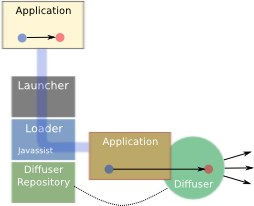
\includegraphics{diffusive_launcher}
\caption{Launching an application in Diffusive}
\label{fig:diffusive_launch_application}
\end{center}
\end{figure}

Figure \ref{fig:diffusive_launch_application} illustrates launching an application in \emph{Diffusive}. At the top of the figure is a box labeled ``Application'' which represents the unadulterated application. The light blue dot in that box represents a method call to the red dot. The red dot represents a \emph{marked} method. The application passes through the launcher and into the loader. The \textsf{DiffusiveLoader} sets up the repository holding the default diffuser, reads the configuration items, creates an \emph{application-attached} diffuser, and hands the application to the Javassist \textsf{Loader} to instrument the application. The tan box labeled ``Application'' in the lower-right hand side of the figure represents the instrumented, or modified, application. Notice that now, all the method calls to the \emph{marked} method are diverted to the \emph{application-attached} diffuser, which contains the required mechanism to execute that method. It is the application-attached diffuser, the green circle on the bottom left-hand side of the figure, that is responsible for distributing the method execution. It is important to point out that the original application code is untouched.

% distributing
\subsubsection{Distributing\label{sec:distributing}}
The \emph{application-attached} diffuser is responsible for distributing method calls to other diffusers, or depending on its configuration and load, executing the method itself. By default \emph{Diffusive} uses a \emph{RESTful} diffuser (\textsf{RestfulDiffuser}) that adheres to the \href{http://jsr311.java.net}{JSR-311} standard\footnote{\url{http://jsr311.java.net}}, and uses the \href{http://jersey.java.net}{Apache Jersey}\footnote{\url{http://jersey.java.net}} implementation. Although \emph{Diffusive} uses a RESTful diffuser by default, any diffuser implementation can be used to provide the required functionality. In fact, \emph{Diffusive} also comes with a local diffuser that runs the code locally\footnote{Using \emph{Diffusive's} local diffuser directly is inefficient. Unless you are using the local diffuser for testing the diffusive framework through a local debugger, using the local diffuser directly means that you aren't diffusing the code. In which case, it doesn't make sense to use \emph{Diffusive} in the first place. The local diffuser only exists because it is used by the RESTful diffuser when it executes a method locally rather than distribute it.}.

The RESTful diffuser must be configured with a set of \emph{end-points} to which it can diffuse method execution. These end-points, themselves, must contain a RESTful diffuser. And the access to the diffuser must be accomplished through a some sort of a software server. \emph{Diffusive} provides a RESTful diffuser server (\textsf{RestfulDiffuserServer}) that contains an \href{http://grizzly.java.net}{Apache Grizzly}\footnote{\url{http://grizzly.java.net}} web server configured to interact with a \href{http://docs.oracle.com/javaee/6/tutorial/doc/giepu.html}{JAX-RS}\footnote{JAX-RS implements JSR-311, providing an implementation for developing RESTful web services in Java. For more information, visit \url{http://docs.oracle.com/javaee/6/tutorial/doc/giepu.html}.} web resource (\textsf{RestfulDiffuserManagerResource}).

Within the context of the RESTful diffuser server, there is one RESTful diffuser for each diffusive method. In other words, each unique diffusive method signature\footnote{A diffusive method signature contains the name of the containing class, the method name, the method's formal argument types, and the return type. This is different from a Java signature, which contains only the method name and the formal argument types.} has its own diffuser, accessible via the web resource (\textsf{RestfulDiffuserManagerResource}) through its uniform resource identifier (URI). The web resource manages the creation, querying, calling, and deletion of its diffusers by responding to requests from the calling diffuser. And each diffuser is a resource with a unique address. For example, a new diffuser is created through an \texttt{HTTP POST} call containing the required information about the diffusive method signature. Obtaining information about a diffuser is accomplished through an \texttt{HTTP GET} call to its URI. To execute a method, an \texttt{HTTP POST} is called on the URI of the diffuser, passing along the information needed to execute the method. The execute method returns an ID (link) to the results resource\footnote{Hypermedia as the engine of application state (HATEOAS).}. The result can then be obtained through an \texttt{HTTP GET} call to the URI of that result, which blocks until the result is complete. Alternatively, the status of the result can be obtained through an \texttt{HTTP HEAD} call to the URI of the result, which is non-blocking, and returns an empty response if the result resource is not yet available. And, finally, a diffuser can be deleted through an \texttt{HTTP DELETE} call to its URI.

To facilitate development, \emph{Diffusive} provides a RESTful client (\textsf{RestfulDiffuserManagerClient}) that takes care of the underlining communication, serializing/deserializing, creating requests, and parsing responses. This client allows developers to deal only with Java objects.

% distribution strategy
\subsubsection{Distribution Strategy\label{sec:distribution_strategy}}
Diffusers decide how to distribute the method calls based on a strategy (\textsf{Strategy}). A \textsf{Strategy} simply returns a list of end-points when requested. In most cases, the list returned by the \textsf{Strategy} contains only one element. However, to allow for redundant diffuser networks, the \textsf{Strategy} interface allows the return of a list of end-points. \textsf{Strategy} implementations can take into account various aspects that affect the optimal distribution of method calls. For example, a \textsf{Strategy} implementation may take into account the load on its server, the number of diffusers executing, the number of threads available for execution, and weighting factors for individual end-points.

% serialization
\subsubsection{Serialization\label{sec:serialization}}
In order to execute a method remotely, the remote execution environment needs certain information. Specifically, the execution environment needs:
\begin{enumerate}
\item The state of the object against which the method call was made.
\item All the arguments to the method.
\end{enumerate}
To transfer that information to the remote diffuser, across the network, they must be serialized. Likewise, once execution is completed, the return object must be serialized and returned to the original diffuser.

When the remote execution environment receives these serialized objects, it must reconstruction them as Java objects. And to reconstruct serialized objects requires Java \textsf{Class} objects corresponding each of the serialized objects. The \textsf{Class} objects are effectively the templates used to reconstruct an object. In section \ref{sec:generic_computation} (\nameref{sec:generic_computation}), we discuss how the remote environment gets access to these \textsf{Class} objects without the need to deploy them prior to execution.

\emph{Diffusive} provides an interface, \textsf{Serializer}, that defines what a serializer must provide to \emph{Diffusive}. Two key serialization implementations have been wrapped to conform to the \textsf{Serializer} interface: \textsf{ObjectSerializer} and \textsf{PersistenceSerializer}. The \textsf{ObjectSerializer} is Java's own serialization framework which requires that classes implement the \textsf{Serializable} interface. Using this serialization framework requires altering existing classes, that are to be serialized, if they don't implement \textsf{Serializable}. In some cases this may be acceptable. In other cases it may not be possible.

The \textsf{PersistenceSerializer} wraps the \href{http://freezedried.sourceforge.net}{FreezeDry} persistence framework\footnote{\url{http://freezedried.sourceforge.net}}. FreezeDry does not require any classes to implement a FreezeDry-specific interface. In fact, FreezeDry can take any existing class (even those without no-arg constructors) and serialize them into XML, JSON, or key-value pairs. However, if the class is too complex, it may require some coding.

% best-efforts failure resolution
\subsection{Best-Efforts Failure Resolution\label{sec:best_efforts_failure_resolution_ref_impl}}
The \emph{Diffusive} reference implementation uses the concept of a \textsf{Strategy} to determine to which diffuser a method is diffused. The current \textsf{Strategy} interface requires that a \textsf{Strategy} return a list of end-points to which the method can be diffused. An implementation of best-efforts failure resolution can be achieved by creating a RESTful diffuser that diffuses its method to the first end-point in the list, and if that fails to the next end-point, until the task completes, or until the diffuser runs out of end-points.

% generic computation
\subsection{Generic Computation\label{sec:generic_computation}}
The \emph{Generic Computation} principle requires two that two conditions are met: that any method can be diffused; and, prior deployment of resources is not required. The first condition is met because of the \emph{Marking} principle---any marked method can be diffused. The second condition is the focus of this section.

As discussed in section \ref{sec:serialization}, \nameref{sec:serialization}, in order to transport objects across the network they must be serialized. This means that to execute a diffusive method remotely requires that the following objects must be serialized:
\begin{enumerate}
\item The object containing the diffusive method.
\item All objects referenced by the object containing the diffusive method.
\item The objects passed to the diffusive method as arguments.
\item All objects referenced by the objects passed to the diffusive method as arguments.
\end{enumerate}
Once these serialized objects are received by the remote diffuser, it needs to deserialize them back into objects. To deserialize any object requires that the class loader has loaded a \textsf{Class} object corresponding to that object (and any objects that object references). Usually, this is handled by deploying the class files (as jar or war files) to the remote servers executing the methods, and configuring their class paths to contain their location.

The \emph{Generic Computation} principle states that deployment of resources to the remote nodes does not need to occur \emph{before} requesting the remote diffuser to execute a method. In practical terms, this principle requires that the remote diffuser contains a mechanism for loading classes from a remote source, and that a mechanism exists, preferably on the application-attached diffuser, that can provide serialized \textsf{Class} objects to the remote diffuser. 

\emph{Diffusive} provides a RESTful class loader (\textsf{RestfulClassLoader}) that can load classes from a corresponding RESTful web service. The \textsf{RestfulClassPathResource} is a (JSR-311) web resource, attached to the web service, that provides serialized \textsf{Class} objects to the requesting client (i.e. the \textsf{RestfulClassLoader}). 

\begin{figure}[htbp]
\begin{center}
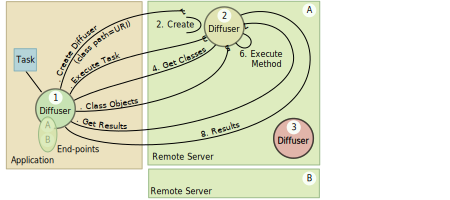
\includegraphics[scale=1.1]{diffusing}
\caption{Process of diffusing a method call}
\label{fig:diffusing}
\end{center}
\end{figure}

Figure \ref{fig:diffusing} shows the process of creating, configuring, and executing a task using \emph{Diffusive}. In this figure, the application requests that its \emph{application-attached} diffuser\footnote{Recall that Javassist is used to redirect calls to methods that were annotated with \textsf{@Diffusive} to the application-aftached diffuser.}, which is labeled as \textsf{Diffuser 1} in the figure, execute the task labeled \textsf{Task}. In this scenario, \textsf{Diffuser 1} decides to diffuse the task to one of its end-points, \textsf{Remote Server A}. If the remote server doesn't contain a diffuser that matches the diffusive method signature of \textsf{Task}, then, as shown in step 1 of figure \ref{fig:diffusing}, \textsf{Diffuser 1} requests that \textsf{Remote Server A} create a diffuser with that signature, which is shown as \textsf{Diffuser 2}. In order to execute \textsf{Task}, \textsf{Diffuser 2} needs to load the \textsf{Class} objects associated with \textsf{Task}. And because \textsf{Diffuser 1} has those \textsf{Class} objects, it passes the URI corresponding to the web service that can provide those \textsf{Class} objects, along with its request to create \textsf{Diffuser 2}.

As shown in step 2 of figure \ref{fig:diffusing}, \textsf{Remote Server A} then creates \textsf{Diffuser 2} and configures it with the class path information and other configuration items, and returns URI to \textsf{Diffuser 2}, the newly created diffuser. \textsf{Diffuser 1} now requests that \textsf{Diffuser 2} execute \textsf{Task} (step 3). As part of that request, \textsf{Diffuser 1} passes all the required serialized object along with the execute request. \textsf{Diffuser 2} receives that request, tries to deserialize the objects, but can't because it doesn't have access to the \textsf{Class} objects associated with \textsf{Task}. And so \textsf{Diffuser 2} initiates a call back to the class path URI requesting the \textsf{Class} objects (step 4).

\textsf{Diffuser 1} sends the serialized \textsf{Class} objects requested back to \textsf{Diffuser 2} (step 5), and \textsf{Diffuser 2} loads the \textsf{Class} objects, which enables it to deserialized the objects associated with \textsf{Task}. Now \textsf{Diffuser 2} is set up to execute the \textsf{Task}, which it does (step 6), and returns a result ID. The result ID is a URI to the result. When \textsf{Diffuser 1} receives the result ID, it requests the result (step 7), which is a blocking call, and waits for the result response (step 8). When \textsf{Diffuser 1} receives the results, it deserialized the result object and returns it the application (again, this is automatic through Javassist).

There are a few noteworthy points. 
\begin{enumerate}
\item Once a diffuser is created, it can be reused, and it can be deleted.
\item The remote class loading is managed through a RESTful class loader and web service, and is part of \emph{Diffusive} by default.
\item When creating a remote diffuser, the class path URI does \emph{not} need to be the URI pointing back to the diffuser requesting the creating. In fact, it can be a common web service that contains a pre-deployed set of class files and can serve them up. However, this reduces the generic computation somewhat.
\end{enumerate}

% indistinguishability and open topology
\subsection{Indistinguishability and Open Topology\label{sec:indistinguishability_and_open_topology}}
In \emph{Diffusive} all diffusers of a certain type are the same. And with the exception of the \emph{application-attached} diffuser, all diffusers are managed the same way. The application-attached diffuser, as the name implies, is attached to the application through the diffusive launcher. Recall that the diffuser launcher is used to launch the application, and during the process of launching the application, the application is instrumented to divert calls to diffusive methods to the application-attached diffuser. It is the application-attached diffuser that diffuses (distributes) method calls to remote diffusers.

\begin{figure}[htbp]
\begin{center}
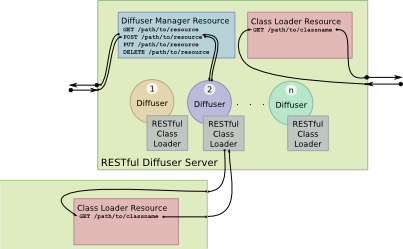
\includegraphics[scale=1.1]{restful_diffuser_server}
\caption{RESTful Diffuser Server}
\label{fig:restful_diffuser_server}
\end{center}
\end{figure}

Recall that in \emph{Diffusive}, a remote diffuser is managed by RESTful diffuser server. A RESTful diffuser servers (\textsf{RestfulDiffuserServer}) act as servers to which methods can be diffused. The RESTful diffuser servers also act as clients when diffusing methods to other remote diffusers, or when other diffusers request \textsf{Class} objects from their class path. And therefore, all remote diffusers look alike. Figure \ref{fig:restful_diffuser_server} shows the basic elements contained in a RESTful diffuser server and depicts a typical interaction. In this scenario, the \textsf{RestfulDiffuserServer} receives a request to execute a method (task). The \textsf{RestfulDiffuserServer}, a web server, forwards the request to the web resource\footnote{A JSR-311 web resource.} (\textsf{RestfulDiffuserManagerResource}) which is bound to its \textsf{execute(...)} method. The execute method looks up the appropriate diffuser based on the diffuser method signature, which is part of the its URI, returns a response containing the result ID (a URI to the result resource) and then forwards the method to that diffuser. 

Each RESTful diffuser contains a \textsf{RestfulClassLoader} which loads a class using a RESTful web service. The \textsf{RestfulClassLoader} acts as a client to the \textsf{RestfulClassPathResource}, which serializes the request \textsf{Class} object and returns it. The RESTful class loader then deserializes the \textsf{Class} object and loads it. Notice that each \textsf{RestfulDiffuserServer} contains the \textsf{RestfulClassPathResource}.

At this point, the diffuser can execute the method and return the result to the \textsf{Restful\-Diffuser\-Manager\-Resource}.

Each diffuser contains a list of end-points to which it can diffuse code, a list of class paths from which it can load \textsf{Class} objects, a \textsf{Strategy} which determines how the end-points for executing the next task are selected, and a RESTful class loader to load class over the network. It is the fact that each diffuser server looks the same that makes each diffuser server a building block from which to construct arbitrary diffuser networks---as long as they can be represented by a directed graph.

%
% Future work
%
\section{Future Work\label{sec:future_work}}
The current reference implementation is a work in progress. The main goal for creating a reference implementation was to prove that the concepts of \emph{diffusive programming} could be implemented, with an eye toward building a robust, secure, and accessible implementation. Given that, there are a number of items that need further exploration and development.

\begin{enumerate}
\item Add best-efforts failure resolution to the RESTful diffuser.
\item Provide additional deployment options (for example, into a servlet container).
\item Create additional diffusers beside RESTful diffusers (for example, RMI diffusers).
\item Create deployment and management tools that allow easy deployment of diffusive servers and allows starting and stopping the diffusive server. Also, allows the management of the diffusers.
\end{enumerate}


\end{document}  